% This file was created with tikzplotlib v0.10.1.
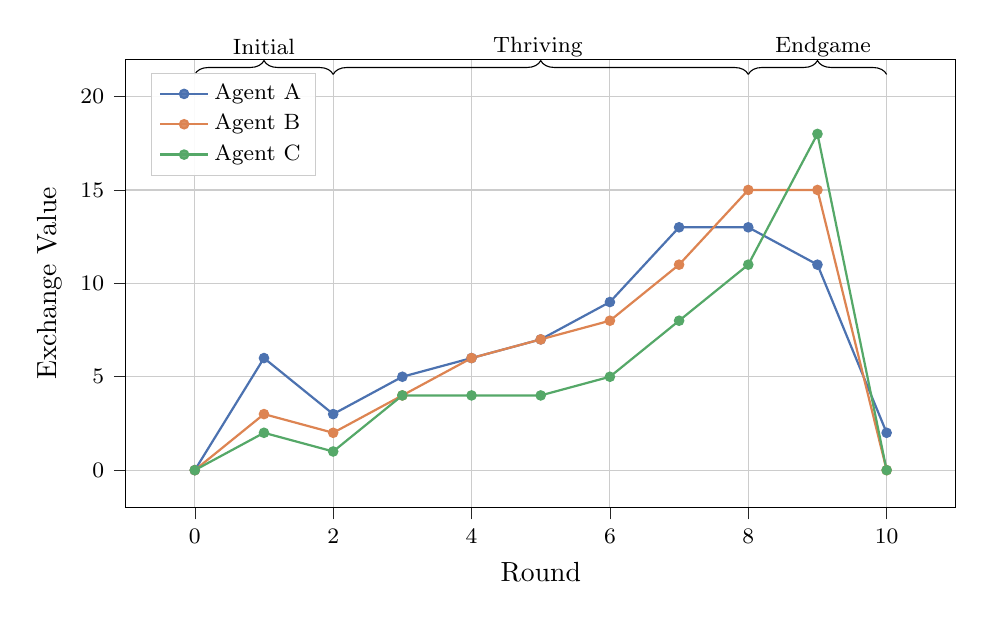
\begin{tikzpicture}

\definecolor{darkorange25512714}{RGB}{221,132,82}
\definecolor{darkslategrey38}{RGB}{38,38,38}
\definecolor{forestgreen4416044}{RGB}{85,168,104}
\definecolor{lightgrey204}{RGB}{204,204,204}
\definecolor{steelblue31119180}{RGB}{76,114,176}


\begin{axis}[
legend cell align={left},
legend style={
  fill opacity=0.8,
  draw opacity=1,
  text opacity=1,
  at={(0.03,0.97)},
  anchor=north west,
  draw=lightgrey204,
  font=\footnotesize
},
width=1.\textwidth,    % 设置宽度
    height=0.6\textwidth,  % 16:9比例
    axis line style={black},
    legend style={fill opacity=0.9, draw opacity=1, text opacity=1, draw=lightgrey204},
    tick align=outside,     % 刻度线向外
    xtick={0,2,4,6,8,10},
    % xticklabels={Initial,Flourishing,Endgame},
     xlabel=Round,
    xlabel style={font=\footnotesize},
    xticklabel style={font=\footnotesize},
    y grid style={lightgrey204},
    ylabel=Exchange Value,
   ylabel style={font=\footnotesize,
            inner sep=0pt,    % 减少标签和轴的距离
            yshift=-12pt       % 微调标签位置
        },
    ymajorgrids,
    ytick={0,5,10,15,20},
    yticklabel style={font=\footnotesize},
    ymin=0, ymax=20,
    xtick style={color=darkslategrey38},
    ytick style={color=darkslategrey38},
    enlarge x limits=0.1,
    enlarge y limits=0.1,
    grid=major,
    grid style={lightgrey204},
    tick style={color=darkslategrey38},
    axis lines=box,        % 保持完整边框
    x axis line style={black},
    y axis line style={black},
    % 控制刻度线的显示
    tick pos=left,         % y轴刻度线只在左侧显示
    xtick pos=bottom,      % x轴刻度线只在底部显示
    clip=false              % 裁剪超出的内容
]
\addplot [thick, steelblue31119180, mark=*, mark size=1.5, mark options={solid}]
table {%
0 0
1 6
2 3
3 5
4 6
5 7
6 9
7 13
8 13
9 11
10 2
};
\addlegendentry{Agent A}
\addplot [thick, darkorange25512714, mark=*, mark size=1.5, mark options={solid}]
table {%
0 0
1 3
2 2
3 4
4 6
5 7
6 8
7 11
8 15
9 15
10 0
};
\addlegendentry{Agent B}
\addplot [thick, forestgreen4416044, mark=*, mark size=1.5, mark options={solid}]
table {%
0 0
1 2
2 1
3 4
4 4
5 4
6 5
7 8
8 11
9 18
10 0
};
\addlegendentry{Agent C}

\draw [decorate, decoration={brace, amplitude=5pt},yshift=8pt] (axis cs:0,20) -- (axis cs:2,20) node [black,midway,yshift=10pt, font=\tiny] {\footnotesize Initial};
\draw [decorate, decoration={brace, amplitude=5pt},yshift=8pt] (axis cs:2,20) -- (axis cs:8,20) node [black,midway,yshift=10pt, font=\tiny,xshift=-1pt] {\footnotesize Thriving};
\draw [decorate, decoration={brace, amplitude=5pt},yshift=8pt] (axis cs:8,20) -- (axis cs:10,20) node [black,midway,yshift=10pt, font=\tiny,xshift=2pt] {\footnotesize Endgame};

\end{axis}

\end{tikzpicture}
